\subsection{Abstract Domains}\label{subsec:abstract-domains}

In the following sections we will describe the abstract domains of our value analysis.

\subsubsection{Abstract domain of strings as regular expressions}\label{subsubsec:abstract_domains_strings}

To represent the abstract domain of the family of SQL strings data types we have chosen regular expressions/languages.
Regular expressions/languages are chosen, as opposed to more powerful representations, for the decidable nature of inclusion and equality between them.

Let $REG$ denote the set of regular languages. % and
% \begin{equation*}
%     REG^{\leq n} = \{R \in REG \mid \forall w \in R : |w| \leq n\}.
% \end{equation*}
In the following we do not distinguish between regular expressions and their languages.

The lattice of $(REG, \subseteq, \cup, \cap)$ is a lattice but not a complete one as the set of regular languages is transfinite and closed under finite union and intersection, but not closed under transfinite union and intersection.
This is a problem: Essentially we can not employ Kleene fixed-point theorem (\autoref{thm:kleene_finite} or \autoref{thm:kleene_scott}) to prove termination of our analysis.

\subsubsection{Abstract domain of numbers as linear inequalities}\label{subsubsec:abstract_domains_numbers}

To represent the abstract domain of the family of SQL number data types when have chosen compound linear inequalities with mixed integer solutions that are algorithmically solvable with MILP solvers (henceforth linear inequalities).
Linear inequalities with mixed integer solutions where chosen for the prevalence and speed of MILP solvers.

Linear inequalities essentially have the same problem as regular expressions. Let $MILP^n$ represent the set of sets of solutions to linear inequalities with $n$ unknowns, then $(MILP^n, \subseteq, \cup, \cap)$ is a non-complete lattice.

\subsubsection{Cover lattice}

The resolve the issue presented above we introduce the notion of a cover lattice, but first we need to define:

\begin{definition}
    A finite non-empty subset $X \subseteq S$ of a lattice $(S, \subseteq, \cup, \cap)$ is called a collectively disjoint top-cover of $S$ whenever $\bigcup X = \top$ and $\bigcap X = \bot$.
\end{definition}

\begin{definition}
    Given a collectively disjoint top-cover $X$ of a lattice $(S, \subseteq, \cup, \cap)$.
    A cover lattice of $S$ in respect to $X$ denoted $\clattice{X}{S}$ is the minimum set where:
    \begin{itemize}
        \item $\forall x \in X: x \in \clattice{X}{S}$,
        \item $\forall x, y \in \clattice{X}{S} : x \cup y \in \clattice{X}{S}$,
        \item $\forall x, y \in \clattice{X}{S} : x \cap y \in \clattice{X}{S}$,
    \end{itemize}
\end{definition}

This gives rise to the following theorem:

\begin{restatable}{theorem}{partition}\label{thm:partition}
    For a non-complete lattice $(S, \subseteq, \cup, \cap)$ and collectively disjoint top-cover $X$ of the cover lattice $(\clattice{X}{S}, \subseteq, \cup, \cap)$ is a finite and complete lattice.
\end{restatable}

And the following lemmas immediately follow:

\begin{lemma}
    If $\mathcal{R}$ is a collectively disjoint top-cover of $(REG, \subseteq, \cup, \cap)$ then $(\clattice{\mathcal{R}}{REG}, \subseteq, \cup, \cap)$ is a complete lattice.
\end{lemma}

\begin{lemma}
    If $X$ is a collectively disjoint top-cover of $(MILP^n, \subseteq, \cup, \cap)$ then $(\clattice{X}{MILP^n}, \subseteq, \cup, \cap)$ is a complete lattice.
\end{lemma}

\begin{example}
    \autoref{fig:tikz-reg-partition} illustrates a simple lattice cover of the regular languages. The regular language $R$ is represented by the gray circle and its complement $\overline{R}$ is represented by the white circle. The union of the two regular language represent the entire regular language $\Sigma^*$ and their intersection is the empty set $\emptyset$.

    \autoref{fig:tikz-reg-partition-lattice} illustrates the cover lattice induced by the lattice cover. The top element $\top$ is the entire regular language $\Sigma^*$ and the bottom element $\bot$ is the empty set $\emptyset$.
\end{example}

% Tikzfigures
\begin{figure}
    \center
    \resizebox{7.5cm}{!}{
        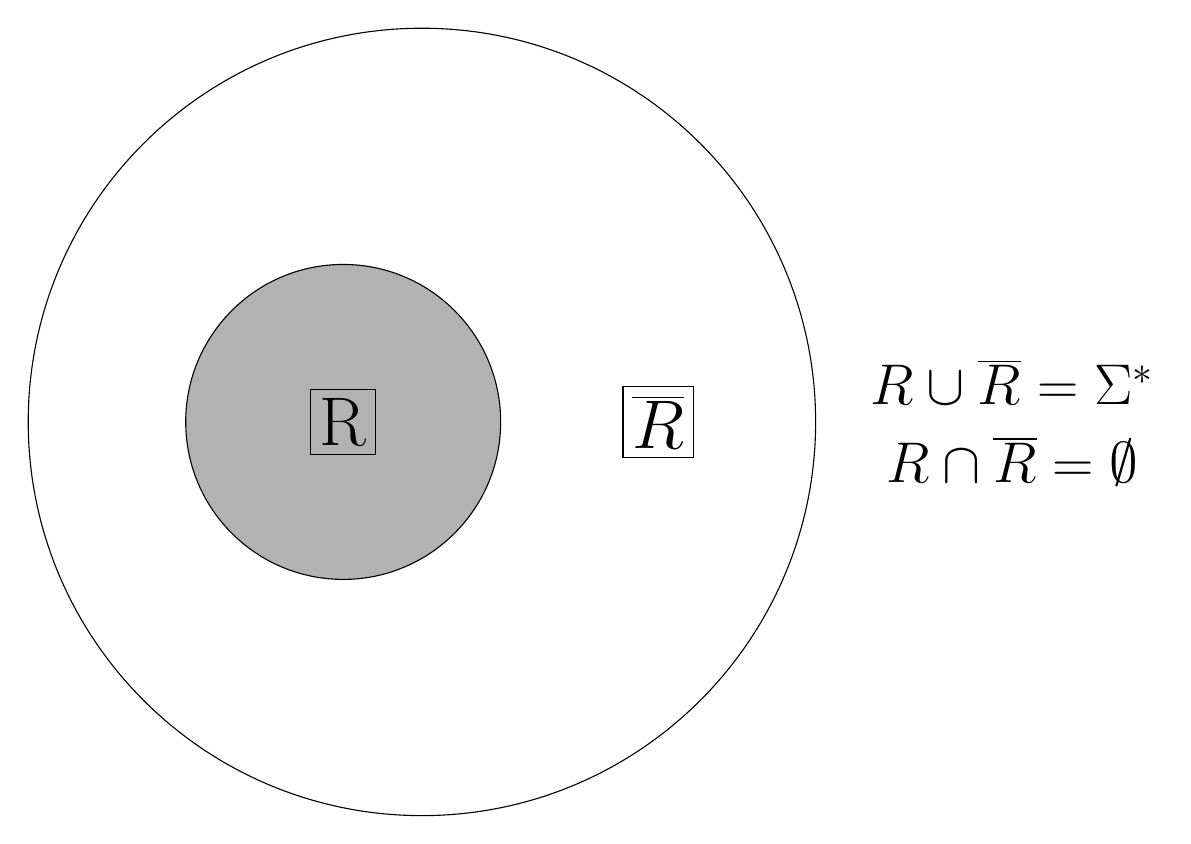
\begin{tikzpicture}
            \filldraw[fill=white, draw=black] (2,2) circle (5cm);
            \node [draw] at (5,2) {\Huge$\overline{R}$};
            \filldraw[fill=gray!60, draw=black] (1,2) circle (2cm);
            \node [draw] at (1,2) {\Huge R};
            \node at (9.5, 2.5) {\huge $R \cup \overline{R} = \Sigma^*$};
            \node at (9.5, 1.5) {\huge $R \cap \overline{R} = \emptyset$};
        \end{tikzpicture}
    }
    \caption{Regular language partition}
    \label{fig:tikz-reg-partition}
\end{figure}


\begin{figure}[!htb]
    \center
    \resizebox{6.5cm}{!}{
        \begin{tikzpicture}[scale = 0.5]
            \usetikzlibrary{calc}
            \node (a) [state] {\Huge$R \cup \overline{R} = \top = \Sigma^*$};
            \node (b1) [state, shift={($(a.south)+(3cm, -2.5cm)$)}] {\Huge $R$};
            \node (b2) [state, shift={($(a.south)+(-3cm, -2.5cm)$)}]{\Huge $\overline{R}$};
            \node (c) [state, shift= {($(a.south) + (0cm, -5.5cm)$)}] {\Huge $R \cap \overline{R} = \bot = \emptyset$};
            \draw (a) to (b1);
            \draw (a) to (b2);
            \draw (b1) to (c);
            \draw (b2) to (c);
        \end{tikzpicture}
    }
    \caption{Regular language partition as a lattice}
    \label{fig:tikz-reg-partition-lattice}
\end{figure}

\subsubsection{Abstract domain of tables}\label{subsubsec:abstract_domain_of_tables}

In the following we consider a table $t$ as function from the domain of possible tuples in the table $\mathbb{T}$ to the codomain of natural (numbers including $0$) $\mathbb{N}$:
\begin{equation}
    t : \mathbb{T} \rightarrow \mathbb{N}.
\end{equation}
The function $t$ describe the number of a given tuple in a table.
We can then consider abstraction over the table $t$ by abstracting either the domain or codomain
This gives rise to a taxonomy of abstract domains of tables shown in \autoref{tab:taxonomy_of_abstract_domain_of_tables}.
In \autoref{tab:taxonomy_of_abstract_domain_of_tables} $\mathbb{T}^\#$ let denote an abstract domain of the set of possible tuples $\mathbb{T}$, such that it forms a finite lattice $(\mathbb{T}^\#, \sqsubseteq, \sqcap, \sqcup)$ (and analogous for $\mathbb{N}$).

\begin{table}
    \caption{Taxonomy of abstract domains of tables}
    \centering
    \begin{tabular}{c|l|c}
    Name & Function & Supported \\
    \hline
    \hline
        Bag of tuples & $\mathbb{T} \rightarrow \mathbb{N}$ & \\
        Abstract bag of tuples & $\mathbb{T} \rightarrow \mathbb{N}^\#$ & \\
        Set of tuples & $\mathbb{T} \rightarrow 2$ & \\
        Bag of abstract tuples & $\mathbb{T}^\# \rightarrow \mathbb{N}$ & \\
        Abstract bag of abstract tuples & $\mathbb{T}^\# \rightarrow \mathbb{N}^\#$ & \checkmark \\
        Set of abstract tuples & $\mathbb{T}^\# \rightarrow \{0, some\}$ & \checkmark \\
        Abstract tuple & $\{\cdot\} \rightarrow \mathbb{T}^\#$ & \checkmark \\
    \end{tabular}
    \label{tab:taxonomy_of_abstract_domain_of_tables}
\end{table}

We will only consider abstract bags of abstract tuples, sets of abstract tuples and abstract tuples because of their finite nature.
In the sequel we will introduce the three abstraction more carefully.

\paragraph{Abstract bag of abstract tuples}

\begin{align*}
    (t \sqcup t')(e) &= t(e) + t'(e) \\
    (t \sqcap t')(e) &= t(e) - t'(e) \\
    t \sqsubseteq t &\iff \forall e \in \mathbb{T}^\# : t(e) \leq t'(e) \\
\end{align*}

If $(\mathbb{N}^\#, \leq, +, -)$ is finite lattice then $(\mathbb{T}^\# \rightarrow \mathbb{N}^\#, \sqsubseteq, \sqcup, \sqcap)$ is a finite lattice.

\paragraph{Set of abstract tuples}

This can be be seen as a specific case of abstract bags of abstract tuples, where the abstract domain $\mathbb{N}^\# = \{0, some\}$ (here some also includes the possibility of $0$) .
We can represent such function as sets, interpreting inclusion to mean the value maps to $some$, and exclusion meaning the value maps to $0$ thus:

\begin{align*}
    t \sqcup t' &= t \cup t' \\
    t \sqcap t' &= t \cap t' \\
    t \sqsubseteq t' &\iff t \subseteq t' \\
\end{align*}

It should be obvious that $(\mathbb{T}^\# \rightarrow \{0, some\}, \sqsubseteq, \sqcup, \sqcap)$ is a finite lattice.

\paragraph{Abstract tuple}

In this case we seek to symbolize the table with just one tuple representing the subsets of the product of it each compound in the tuple.

\begin{align*}
    (t \sqcup t')(\cdot) &= t(\cdot) \sqcup t'(\cdot) \\
    (t \sqcap t')(\cdot) &= t(\cdot) \sqcap t'(\cdot) \\
    t \sqsubseteq t' &\iff t(\cdot) \sqsubseteq t'(\cdot) \\
\end{align*}

It should be obvious that $(\{\cdot\} \rightarrow \mathbb{T}^\#, \sqsubseteq, \sqcup, \sqcap)$ is a finite lattice.
